\documentclass[../portafolio.tex]{subfiles}

\begin{document}

\chapter{Cálculo de una integral usando series} 

\hfill \textbf{Fecha de la actividad:} 13 de septiembre de 2022

\medskip

%---------------------------------------------------------------------------------
% Introducción/objetivos de la actividad
En esta actividad, buscamos evaluar integrales de la forma:
\begin{align}
  \label{eq:In_series_quadrature}
  I_n = \int_0^1 dx\, x^n \sin x \,,
\end{align}
%
para lo cual usaremos dos estrategias distintas: Evaluaremos la ecuación \eqref{eq:In_series_quadrature} usando la regla del trapezoide, y; manipularemos la ecuación \eqref{eq:In_series_quadrature} para encontrar una ley de recurrencia.

%---------------------------------------------------------------------------------
% Selección de evidencias
\section{Regla trapezoidal}
Según la regla trapezoidal, aproximamos la ecuación \eqref{eq:In_series_quadrature} como:
\begin{align}
  \label{eq:In_quad_trapz}
  I_n = \int_0^1 dx\,f(x) \simeq \frac{1}{N} \left[ \frac{f(x_0) + f(x_N)}{2} + \sum_{k=1}^{N-1} f(x_k)  \right] \,,
\end{align}
%
donde $f(x)=x^n \sin x$, $x_k=k/N$, y $N$ es el número de subintervalos entre $x=0$ y $x=1$. La ecuación \eqref{eq:In_quad_trapz} puede ser evaluada usando un código similar al que sigue: 
\begin{pythoncode}
  x = numpy.linspace(0, 1, Nmax)   # elige $N_\text{max}$ valores de $0<x<1$
  fk = f(x, n)                  # evalúa $f(x)$ para cada $x$ y cierto valor de $n$
  
  # evalúa \eqref{eq:In_quad_trapz}
  In = (0.5*(fk[0] + fk[-1]) + np.sum(fk[1:-1])) / Nmax
\end{pythoncode}

\section{Evaluación mediante series}
Integrando (\ref{eq:In_series_quadrature}) por partes dos veces, se tiene que:
\begin{align*}
  I_n
  &= -x^n \cos x\Bigg|_0^1 + \int_0^1 dx\, n x^{n-1} \cos x  \,, \\
  &= (-x^n \cos x + n x^{n-1} \sin x) \Bigg|_0^1 - \int_0^1 dx\, n (n-1) x^{n-2} \sin x  \,.
\end{align*}

Usando (\ref{eq:In_series_quadrature}) para definir $I_{n-2}$ y
teniendo precaución con los casos particulares $n=0$ y $n=1$,
encontramos:
\begin{align}
  \label{eq:In_series_partes}
  I_n
  &=
    \begin{cases}
      1 -\cos(1) & n=0  \\
      \sin(1)-\cos(1) & n=1 \\
    -\cos(1) + n \sin(1) - n (n-1) I_{n-2} & n\geq 2     
    \end{cases}
    \,.
\end{align}

Es decir, conocidos $I_0=1 -\cos(1)$ e $I_1=\sin(1)-\cos(1)$, podemos
usarlos como semillas para calcular todos los valores de $I_n$ con
$n\geq2$, lo cual hacemos usando un código similar al que sigue: 
\begin{pythoncode}
  # Como necesitamos evaluar varias veces $\cos(1)$ y $\sin(1)$, es
  # mejor guardar sus valores para no volver a evaluar tales funciones
  cos1, sin1 = np.cos(1), np.sin(1)

  # Podemos reservar inmediatamente memoria para calcular los primeros
  # $N$ elementos de la serie $I_n$
  In = np.zeros(N)
  
  # Evaluamos las semillas $I_0$ e $I_1$
  In[0] = 1 - cos1
  In[1] = sin1 - cos1
  
  # evaluamos $I_n$ para $2\leq n < N$
  for n in range(2,N):
      In[n] = n*sin1 - cos1 - n*(n-1)*In[n-2]
\end{pythoncode}


En la figura \ref{fig:In_series_trapz} se muestran los resultados de
evaluar $I_n$ según la regla trapezoidal \eqref{eq:In_quad_trapz}
usando $N=100$ nodos entre $0\leq x \leq 1$; y mediante la relación de
recurrencia \eqref{eq:In_series_partes}. Observamos pequeñas
diferencias entre las dos aproximaciones, especialmente para $n=0$ y
$n=1$. Sin embargo, notemos que $I_0=1 -\cos(1)$ e
$I_1=\sin(1)-\cos(1)$ son valores exactos de las integrales
correspondientes. Por lo tanto, se puede concluir que la regla
trapezoidal no es lo suficientemente precisa y se sugiere usar
valores de $N$ mayores para mejorar la aproximación.
\begin{figure}[ht!]
  \centering
  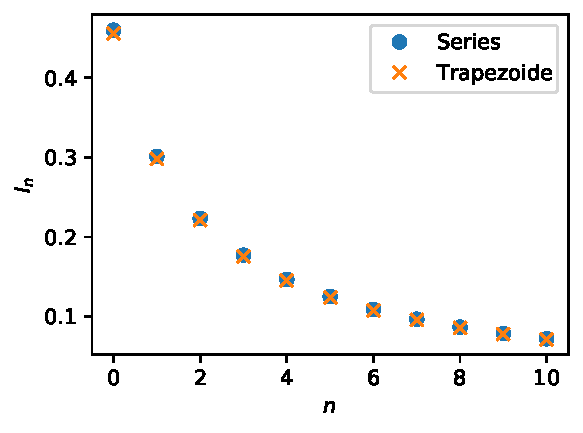
\includegraphics[width=0.5\textwidth]{In_series_trapz}
  \caption{Valores de $I_n$ definido en \eqref{eq:In_series_quadrature} para distintos valores de $n$ según el método trapezoidal \eqref{eq:In_quad_trapz} y la relación de recurrencia \eqref{eq:In_series_partes}. El código para crear esta figura se encuentra en \href{src/0913-series/grafica\_In\_series\_trapz.py}{src/0913-series/grafica\_In\_series\_trapz.py}}
  \label{fig:In_series_trapz}
\end{figure}
  


\end{document}
